% !TeX root = ../main.tex

% \chapter{研究点1 }

% \section{RIS 的工作原理与技术特性}


% \section{图片示例}

% 我们分析了一个MU-MIMO系统,该系统包括一个基站(Base Station, BS)、一个RIS和多个用户。基站配备了$N_t$个天线。每个用户拥有$N_r$个天线,而RIS由$L$个被动元件组成,由RIS控制器进行控制。RIS的反射元件均匀分布在一个平面矩形阵列中。该系统使用长期统计CSI来优化传输,而无需实时反馈。如图\ref{fig:system}所示。

% \begin{figure}[ht]
%   \centering
%   
\includegraphics[width=\textwidth]{nwnulog.png}
%   \caption{Logo}
%   \label{fig:logo}
%   % \note{注:图注的内容不宜放到图题中。}
% \end{figure} 

% 假设基站到用户的直传路径被物理障碍物(如建筑物)遮挡。RIS上的每个反射单元能够调整入射电磁波的相位偏移,由RIS控制器管理。
% 设$\mathbf{H}_{\mathrm{1}}\in\mathbb{C}^{L \times N_t}$表示基站到RIS的信道矩阵,$\mathbf{H}_{\mathrm{2,K}}\in\mathbb{C}^{N_r \times L}$表示RIS到第$k$个用户的信道矩阵,则基站到第$k$个用户的整体级联信道$\mathcal{H}_{k}$可表示为:
% \begin{equation}
%   \mathcal{H}_{k} = \mathbf{H}_{1}\bm{\Phi}\mathbf{H}_{2,k},
%   \label{eq:cascadechannel}
% \end{equation}

% $\bm{\Phi} = \text{diag}(e^{j\theta_1}, e^{j\theta_2}, ..., e^{j\theta_L})$ 是由RIS引入的相移的对角矩阵,$\boldsymbol{\theta} = [\theta_1, \theta_2, ..., \theta_L]^T$ 表示相移,其中 $\theta_l \in [0, 2\pi]$ 为第$l$个RIS单元的相移。
% 在实际的传播环境中,用户设备、基站和RIS上天线和反射单元的密集部署会引起空间相关性。这种相关性显著影响可实现的通信速率,特别是在考虑到设备和表面尺寸有限的情况下。为了建模空间相关性的影响,信道矩阵$\mathbf{H}_{1}$和$\mathbf{H}_{2,k}$采用广泛使用的克罗内克相关信道模型[23],如下所示:

% \begin{equation}
%   \mathbf{H}_{1}=\sqrt{\beta_{1}}\Sigma_{R_{I}}^{\frac12}\tilde{\mathbf{H}}_{1}\Sigma_{TB}^{\frac12},
% \end{equation} 
% \begin{equation}
%   \mathbf{H}_{2,k}=\sqrt{\beta_{2}}\Sigma_{R_{2,k}}^{\frac{1}{2}}\tilde{\mathbf{H}}_{2,k}\Sigma_{T_{I}}^{\frac{1}{2}}, k\in\{1,\cdots,K\}.
% \end{equation}


% 具体来说,$\beta_{1}^{\frac12}$和$\beta_{2,k}^{\frac12}$表示长期路径损耗效应,$\tilde{\mathbf{H}}_{1}$和$\tilde{\mathbf{H}}_{2,k}$是随机矩阵,其元素是独立同分布(i.i.d.)的复值圆形对称高斯随机变量,
% 确定性协方差矩阵$\Sigma_{T_{1}}$、$\Sigma_{R_{2,k}}$、$\Sigma_{T_{I}}$和$\Sigma_{R_{I}}$用于表征发射天线、接收天线和RIS元件之间的空间相关性,这些协方差矩阵被假设为半正定的厄米特矩阵。
% 为简化分析,这些空间相关矩阵被认为是时不变的,因为空间相关性通常在较长时间内保持稳定,主要由MIMO天线配置、RIS反射元件和工作频率决定。
% 基站发射的信号用$\mathbf{x}$表示,第$k$个用户的噪声遵循复值高斯分布,方差为$\sigma_k^2$:$\mathbf{n}_k \sim \mathcal{CN}(\mathbf{0}, \sigma_n^2 \mathbf{I}_{N})$基站发射的整体信号$\mathbf{x}$由所有用户的数据组成。最终的整体发射信号可以表示为:

% \begin{equation}
%   \mathbf{x}=\sum_{k=1}^K\mathbf{x}_k=\sum_{k=1}^K\mathbf{B}_k\mathbf{d}_k=\mathbf{B}\mathbf{d},
% \end{equation}

% $\mathbf{B}_{k} \in \mathbb{C}^{N_t \times N_r }$和$\mathbf{d}_{k} \in \mathbb{C}^{N_r \times 1}$分别是第$k$个用户的波束赋形矩阵和数据符号,
% 整体波束赋形矩阵和符号向量分别为:$\mathbf{B} = [\mathbf{B}_{1}, \mathbf{B}_{2}, \ldots, \mathbf{B}_{K}]$。与其他研究不同,这里的波束赋形设计涉及多个波束$\mathbf{B} \in \mathbb{C}^{N_t \times N_r \times K}$,符号向量为$\mathbf{d} = [\mathbf{d}_{1}^{T}, \mathbf{d}_{2}^{T}, \ldots, \mathbf{d}_{K}^{T}]^{T}$,假设数据符号是无关的$\mathbb{E}[\mathrm{dd}^\mathrm{H}]=\mathbf{I}_{KN_r}$。
% 第$k$个用户接收到的信号可通过以下方程表示:

% \begin{equation}\label{equ:yk}
%   \mathbf{y}_k=\mathcal{H}_k^\mathrm{H}\mathbf{x}+\mathbf{n}_k,
% \end{equation}

% $\mathbf{x}$表示从基站发射的信号向量,$\mathbf{n}_k$表示第$k$个用户接收器处的噪声向量。


% \section{算法实例}

% 模板中使用 \pkg{algorithm2e} 宏包实现算法环境。关于该宏包的具体用法,
% 请阅读宏包的官方文档。

% \begin{algorithm}
%   % \SetAlgoLined  # 增加竖线
%   \KwIn{this text}
%   \KwOut{how to write algorithm with \LaTeX2e }
%   \algline
%   initialization\;
%   \While{not at end of this document}{
%     read current\;
%     \eIf{understand}{
%       go to next section\;
%       current section becomes this one\;
%     }{
%       go back to the beginning of current section\;
%     }
%   }
%   \caption{算法示例1}
%   \label{algo:algorithm3}
% \end{algorithm}



% 注意,我们可以在论文中插入算法,但是插入大段的代码是愚蠢的。
% 然而这并不妨碍有的同学选择这么做,对于这些同学,建议用 \pkg{listings} 宏包。

% \section{数值结果和分析}
% 在本节中,我们展示了基于假设场景进行的数值仿真。仿真设置包括一个基站与四个用户的通信,并由RIS辅助。仿真中考虑了统计CSI和空间相关性。对于基站和用户采用的均匀线性阵列拓扑结构,相关矩阵  和  的第 元素分别为   和  ,其中 。
% 对于RIS,我们假设 ,并使用垂直和水平相关矩阵的克罗内乘积来建模RIS的相关性。设备之间的相关系数设置为 ,表示相邻天线或反射元件之间的相关系数。
% 经过训练过程后,最终参数选择由表 1给出,其选值基于训练结果进行了进一步优化,以实现系统性能的提升。

% \begin{table}
%   \centering
%   \caption{系统仿真参数}
%   \label{tab:paramater8}
%   \begin{tabular}{cll}
%     \toprule
%     类型   & 描述                                     & 描述   \\
%     \midrule
%     挂线表 & 挂线表也称系统表、组织表,用于表现系统结构   & 描述    \\
%     无线表 & 无线表一般用于设备配置单、技术参数列表等     & 描述    \\
%     卡线表 & 卡线表有完全表,不完全表和三线表三种         & 描述    \\
%     \bottomrule
%   \end{tabular}
% \end{table}

% 值得注意的是,由于(17)以及(18)白化和动作归一化,我们的DRL方法通过直接在单次训练中获取状态和动作,实现了高效的学习和更快的收敛。这一过程增强了模型的泛化能力,使得在低SNR环境下,相较于其他基准方法,能够获得更高的速率。
% 如图 2所示。随着SNR的增加,所有方法的速率和都呈逐渐上升趋势。在低信噪比时,提出的DRL方案相较于BCD、AO和随机相位三种基准方法,表现出更好的效果,随着信噪比的增加,各方法之间的差距逐渐减小,且AO方法的性能优于随机相位方法,而BCD方法优与AO方法。


% 我们研究了发射功率 对训练以及系统性能的影响。如图 3所示,在较低的传输功率(  = 5 dB)下,瞬时奖励表现出较高功率下更平缓的波动性,但整体奖励值较低,平均奖励呈现平滑上升趋势。而在较高的传输功率(  = 30 dB)下,瞬时奖励表现出较大的波动性,随着时间步长的增加,波动逐渐减小,相应的平均奖励呈现比5dB更好的上升趋势,最后逐渐趋于平稳。

% 总体而言,较高的发射功率不仅带来更高的奖励值,还加速了奖励的收敛过程,而较低的发射功率则导致较低的奖励水平和较慢的收敛速度。

% 如图 4所示,更多的天线能够显著提升和速率的基线值和上限,而反射元件数量的增加则在初期带来显著的性能增益,但随着RIS元素数量 的增加,RIS通信系统的总速率逐渐达到饱和点。这一结果突出了我们的DRL方法的有效性,因为它能够高效地适应更大的RIS配置。值得注意的是,系统在没有显著增加收敛时间的情况下,继续提供最优性能,展示了DRL方法的鲁棒性和可扩展性。



\chapter{研究点1:MIMO通信系统建模}

\section{MIMO系统概述}

多输入多输出(MIMO)技术通过在发射端和接收端使用多个天线,显著提高无线通信系统的频谱效率和数据速率 \cite{cho2010mimo}。MIMO系统利用空间分集和多路复用增益,能够在不增加带宽的情况下提升通信性能。本节介绍一个简化的MIMO系统模型,分析其信道特性和性能。

\section{系统模型}

考虑一个点到点的MIMO系统,基站(BS)配备 \( N_t \) 个发射天线,接收用户配备 \( N_r \) 个接收天线。假设信道为平坦瑞利衰落信道,信道矩阵 \(\mathbf{H} \in \mathbb{C}^{N_r \times N_t}\) 的元素为独立同分布的复高斯随机变量,服从 \(\mathcal{CN}(0, 1)\)。

发射信号向量为 \(\mathbf{x} \in \mathbb{C}^{N_t \times 1}\),接收信号向量 \(\mathbf{y} \in \mathbb{C}^{N_r \times 1}\) 可表示为:
\begin{equation}
  \mathbf{y} = \mathbf{H} \mathbf{x} + \mathbf{n},
  \label{eq:mimo_channel}
\end{equation}
其中 \(\mathbf{n} \in \mathbb{C}^{N_r \times 1}\) 为加性高斯白噪声,服从 \(\mathcal{CN}(\mathbf{0}, \sigma^2 \mathbf{I}_{N_r})\),\(\sigma^2\) 为噪声方差。

为提高系统性能,基站采用预编码技术,发射信号为 \(\mathbf{x} = \mathbf{P} \mathbf{s}\),其中 \(\mathbf{P} \in \mathbb{C}^{N_t \times N_s}\) 为预编码矩阵,\(\mathbf{s} \in \mathbb{C}^{N_s \times 1}\) 为数据符号向量,\(N_s \leq \min(N_t, N_r)\) 为数据流数量。假设数据符号满足 \(\mathbb{E}[\mathbf{s} \mathbf{s}^H] = \mathbf{I}_{N_s}\)。

系统的信道容量可通过以下公式计算:
\begin{equation}
  C = \log_2 \det \left( \mathbf{I}_{N_r} + \frac{1}{\sigma^2} \mathbf{H} \mathbf{P} \mathbf{P}^H \mathbf{H}^H \right),
  \label{eq:capacity}
\end{equation}
其中 \(\det(\cdot)\) 表示矩阵行列式,\(\mathbf{P}^H\) 为预编码矩阵的共轭转置。

\section{系统示意图}

\begin{figure}[ht]
  \centering
  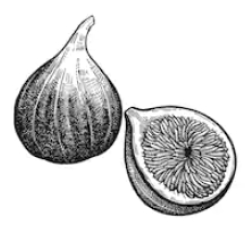
\includegraphics[width=0.8\textwidth]{fig_sample.png}
  \caption{示例图片}
  \label{fig:mimo_sample}
\end{figure}

如图 \ref{fig:mimo_sample} 所示,MIMO系统通过多天线配置实现多路并行数据传输,显著提升吞吐量。

\section{算法示例}

以下的算法\ref{algo:algorithm_sample}展示一个简单的算法示例。

\begin{algorithm}
  \KwIn{this text}
  \KwOut{how to write algorithm with \LaTeX2e }
  \algline
  initialization\;
  \While{not at end of this document}{
    read current\;
    \eIf{understand}{
      go to next section\;
      current section becomes this one\;
    }{
      go back to the beginning of current section\;
    }
  }
  \caption{算法示例1}
  \label{algo:algorithm_sample}
\end{algorithm}



\section{仿真参数}

为验证系统性能,仿真中采用以下参数设置:

\begin{table}[ht]
  \centering
  \caption{MIMO系统仿真参数}
  \label{tab:mimo_parameters}
  \begin{tabular}{llc}
    \toprule
    参数 & 描述 & 值 \\
    \midrule
    \(N_t\) & 发射天线数 & 4 \\
    \(N_r\) & 接收天线数 & 4 \\
    \(N_s\) & 数据流数 & 2 \\
    \(\sigma^2\) & 噪声方差 & 0.1 \\
    \(P_t\) & 发射功率 & 1 W \\
    \bottomrule
  \end{tabular}
\end{table}